\documentclass[a4paper]{jpconf}
\usepackage{graphicx}
\usepackage{lineno}
\linenumbers
\bibliographystyle{iopart-num}
\usepackage{amssymb, amsmath}
\usepackage{hyperref}

\DeclareMathOperator*{\argmin}{arg\,min}
\DeclareMathOperator*{\argmax}{arg\,max}
\begin{document}
\title{Approximating and decomposing likelihood ratios on mixture models using machine learning}
%\title{Approximating decomposed likelihood ratios using machine learning}

\author{K Cranmer$^1$, J Pavez$^2$,
G Louppe$^1$\ and  W Brooks$^3$}

\address{$^1$ Physics Department, New York University, New York, NY 10003, U.S.A.}
\address{$^2$ Informatics Department, Universidad T\'ecnica Federico Santa Mar\'ia, 1240 Av. Espa\~na, Valpara\'iso, Chile}
\address{$^3$ Physics Department, Universidad T\'ecnica Federico Santa Mar\'ia, 1240 Av. Espa\~na, Valpara\'iso, Chile}

\ead{juan.pavezs@alumnos.usm.cl}


\begin{abstract}
Likelihood ratio test are a key tool in many fields of science. In order to evaluate the likelihood ratio the likelihood function is needed. However, it is common in fields like high energy physics to have complex simulations that describe the distribution while not having a description of the likelihood that can be directly evaluated. In this setting it is impossible or computationally expensive to evaluate the likelihood. It is possible to construct an equivalent version of the likelihood ratio that can be easily evaluated by using discriminative classifiers. We show how this can be used to approximate the likelihood ratio when the underlying distribution is a weighted sum of probability distributions (e.g. signal plus background model). We demonstrate how the results can be considerably improved by decomposing the test and use a set of classifiers in a pairwise manner on the components of the mixture model and in which way this can be used to estimate the unknown coefficients of the model, such as the signal contribution.
\end{abstract}
\section{Introduction}

In High Energy Physics (HEP) and many other fields hypothesis testing is a key tool when reporting results from an experiment. Likelihood ratio tests are 
the main technique for hypothesis testing and they are the most powerful statistic for simple hypothesis testing. For composite hypothesis 
testing the profile or generalized likelihood ratio test is commonly used. When computing the likelihood ratio the data distribution $p(x|\theta)$ must 
be evaluated, where $\theta$ are parameters of the probability distribution. However, it is common in HEP to have physics simulations that allow to sample high dimensional vectors from the distribution $p(x|\theta)$ while not having a description that can be directly evaluated. Commonly it is impossible or computationally expensive to evaluate the likelihood ratio in this setting. % as a high dimensional vector while not having a description that can be directly evaluated. This simulations are used to obtain a high dimensional observation $x$ by emulating the underlying physics of the process. Commonly it is impossible or computationally expensive to evaluate the likelihood ratio in this setting.

A common use of likelihood ratios in HEP is signal process identification. In this task the hypothesis testing procedure is used to evaluate the signal process significance by contrasting the only background (null) hypothesis versus the signal plus background (alternative) hypothesis. In this setting, the underlying distribution can be seen as a signal and background mixture model defined as
\begin{equation}\label{eq:sigbkg}
p( x \,|\, \mu, \nu) =  \mu p_s( x \, |\,  \nu)  + (1-\mu)\, p_b( x \,|\, \nu) ,
\end{equation}
where $p_x(x \, |\, \nu)$ correspond to the signal distribution and $p_b(x \, |\, \nu)$ is the background distribution, both parametrized by nuisance parameters $\nu$ which describe uncertainties in the underlying physics predictions or response of measurement devices. The parameter $\mu$ is the mixture coefficient corresponding to the signal component of the distribution. In this case the generalized likelihood ratio test takes the form of 
\begin{equation}
\lambda(D) = \prod_{e=1}^n \frac{ p(x_e|\mu=0,\hat{\hat{\nu}})}{ p(x_e|\hat \mu, \hat \nu)},
\end{equation}
where $D$ is a data set of i.i.d observations $x_e$, $\hat {\hat \nu}$ is the conditional maximum likelihood estimator for $\nu$ under the null hypothesis $\theta_0$ ($\mu = 0$) and $\hat{\nu}, \hat{\mu}$ are the maximum likelihood estimators for $\nu$ and $\mu$. This approach has been used extensively to assert the discovery of new particles in HEP~\cite{Cowan:2010js}, such as in the discovery of the Higgs boson~\cite{Aad:2012tfa,Chatrchyan:2012ufa}.

%It has been recently proved that discriminative classifiers can be used to solve this problem by constructing an equivalent version of the likelihood ratio in this likelihood-free setting~\cite{Cranmer2015}.
As previously mentioned, the original distributions for signal and background can only be approximated by forward simulations. Most of the likelihood ratio tests at the LHC are made on the distribution of a single feature that discriminate between signal and background observations. For this, the simulated data is used together with interpolations algorithms in order to approximate the parametrized model and then use it in the hypothesis testing procedure~\cite{Cranmer:2012sba}.

%To obtain a discriminative feature between signal and background various experiments use supervised learning methods by training a discriminative classifier which can learn to classify between signal and background given the original high-dimensional simulated data. In HEP methods like boosted decision trees and multilayer perceptron has been implemented in libraries such as TMVA and used extensively~\cite{Hocker:2007ht}.

Noticeably, it has been shown that a discriminative classifier trained to classify between signal and background can be used to obtain an equivalent likelihood ratio test~\cite{Cranmer2015}. Given a classifier trained to learn a monotonic function of the per event ratio $p(x_e | \theta_0) / p(x_e | \theta_1)$(this is the usual case since many of the commonly used classifiers learn to approximate some monotonic function of the regression function), the likelihood ratio test on the conditional distributions of the score is equivalent to the original likelihood ratio.

In this work we show how these results can be used to approximate the likelihood ratio when the underlying distribution is a weighted sum of probability distributions (mixture model). %This case is common in physics when identifying a signal process over one or more background process. 
We also show that by training a set of classifiers in a pairwise manner on the components of the mixture model it is possible to improve considerably the results of the approximation. %Finally, we demonstrate how this technique can also be used to estimate the unknown weights coefficients in the mixture model or equivalently the signal and background respective contributions.

%This note is organized as follows. Section~\ref{S:ALR} gives a brief overview of how likelihood ratios are used at the LHC and how this ratios can be approximated by using supervised learning techniques. In Section~\ref{S:DLR} the method to approximate likelihood ratios on mixture models is explained and in Section 4 a study of the results obtained by the algorithm on toy distributions is presented.

%\section{Approximating likelihood ratios using discriminative classifiers}\label{S:ALR}
%\subsection{}

%A common use of likelihood ratios in HEP is signal process identification. In this task the hypothesis testing procedure is used to evaluate the signal process significance by contrasting the only background (null) hypothesis versus the signal plus background (alternative) hypothesis. In this setting, the underlying distribution can be seen as a signal and background mixture model defined as
%\begin{equation}\label{eq:sigbkg}
%p( x \,|\, \mu, \nu) =  \mu p_s( x \, |\,  \nu)  + (1-\mu)\, p_b( x \,|\, \nu) ,
%\end{equation}
%where $p_x(x \, |\, \nu)$ correspond to the signal distribution and $p_b(x \, |\, \nu)$ is the background distribution, both parametrized by nuisance parameters $\nu$ which describe uncertainties in underlying physics predictions or response of measurement devices. The parameter $\mu$ is the mixture coefficient corresponding to the signal component of the distribution. In this case the generalized likelihood ratio test takes the form of 
%\begin{equation}
%T(D) = \prod_{e=1}^n \frac{ p(x_e|\mu=0,\hat{\hat{\nu}})}{ p(x_e|\hat \mu, \hat \nu)},
%\end{equation}
%where $D$ is a data set of i.i.d observations $x_e$, $\hat {\hat \nu}$ is the conditional maximum likelihood estimator for $\nu$ under the null hypothesis $\theta_0$ ($\mu = 0$) and $\hat{\nu}, \hat{\mu}$ are the maximum likelihood estimators for $\nu$ and $\mu$. This approach has been used extensively to assert the discovery of new particles in HEP~\cite{Cowan:2010js}, such as in the discovery of the Higgs boson~\cite{Aad:2012tfa,Chatrchyan:2012ufa}.

%As previously mentioned, the original distributions for signal and background can only be approximated by forward simulations. Most of the likelihood ratio tests at the LHC are made on the distribution of a single feature that discriminate between signal and background observations. For this, the simulated data is used together with interpolations algorithms in order to approximate the parametrized model and then use it in the hypothesis testing procedure~\cite{Cranmer:2012sba}.

%To obtain a discriminative feature between signal and background various experiments use supervised learning methods by training a discriminative classifier which can learn to classify between signal and background given the original high-dimensional simulated data. In HEP methods like boosted decision trees and multilayer perceptron has been implemented in libraries such as TMVA and used extensively~\cite{Hocker:2007ht}.

%Noticeably, it has been shown that a discriminative classifier trained to classify between signal and background can be used to obtain an equivalent likelihood ratio test~\cite{Cranmer2015}. Given a classifier trained to learn a monotonic function of the per event ratio $p(x_e | \theta_0) / p(x_e | \theta_1)$(this is the usual case since many of the commonly used classifiers learn to approximate some monotonic function of the regression function), the likelihood ratio test on the conditional distributions of the score is equivalent to the original likelihood ratio.

%Let  $s(x;\theta_0, \theta_1)$ to represent the classification score learned by the classifier, parametrized by $\theta_0$ and $\theta_1$ the parameters of the statistical model, let $p( s({x; \theta_0, \theta_1}) | \theta )$ the probability distribution of the score on the data from the original distribution $p(x | \theta)$. Then, the likelihood ratio test is equivalent to the test on the conditional distributions of the score, 
%\begin{equation}\label{eq:lrtest}
%T(D) = \prod_{e=1}^n \frac{ p(x_e | \theta_0)}{ p(x_e | \theta_1)} = \prod_{e=1}^n \frac{ p(s(x_e; \theta_0, \theta_1) | \theta_0)}{ p(s(x_e; \theta_0, \theta_1) | \theta_1)},
%\end{equation}
%where $\theta_0$ correspond to the null hypothesis and $\theta_1$ to the alternative hypothesis. The only requirement is that the discriminative classifier learns a monotonic function of the per event ratio $p(x_e | \theta_0) / p(x_e | \theta_1)$~\cite{Cranmer2015}. This is the usual case since many of the commonly used classifiers learn to approximate some monotonic function of the regression function $s(x) \sim p(y|x) = p(x|\theta_1) / (p(x|\theta_0) + p(x|\theta_1))$ which is monotonic to the desired ratio. %[Tishbshirani].
 
 %In the next section we show how this result can be used to decompose a likelihood ratio for mixture models into the likelihood ratio of its components obtained by training a set of classifiers pairwise.
 
\section{Decomposed likelihood ratio test for mixture models}\label{S:DLR}
A generalized version of the signal and background mixture  model of eq.~(\ref{eq:sigbkg}) for several components is 
\begin{equation}
p(x|\theta)=\sum_{i=1}^k w_i(\theta) p_i(x|\theta),  
\end{equation}
where $w_i(\theta)$ are the mixture coefficients for each one of the components parametrized by $\theta$. In~\cite{Cranmer2015} it is shown that the likelihood ratio between two mixture models
\begin{equation}
\frac{p(x|\theta_0)}{p(x|\theta_1)}= \frac{ \sum_{i=1}^k  w_i(\theta_0) p_i(x|\theta_0)}{\sum_{j=1}^{k'} w_{j}(\theta_1) p_{j}(x| \theta_1)}, 
\end{equation}
is equal to the composition of pairwise ratios for each one of the components which is equivalent to the composition of ratios on the score distribution of pairwise trained classifiers
\begin{equation}\label{eq:decomp}
\frac{p(x|\theta_0)}{p(x|\theta_1)} = \sum_{i=1}^k \left[ \sum_{j=1}^{k'} \frac{ w_{j}(\theta_1)}{w_i(\theta_0)} \frac{ p_{j}(x|\theta_1)}{  p_i(x| \theta_0)}  \right]^{-1} = \sum_{i=1}^k \left[ \sum_{j=1}^{k'} \frac{ w_{j}(\theta_1)}{w_i(\theta_0)} \frac{ p_{j}(s_{i,j}(x;\theta_0, \theta_1)|\theta_1)}{  p_i(s_{i,j}(x;\theta_0, \theta_1)| \theta_0)}  \right]^{-1}.
\end{equation}
In the case that the only free parameters of the mixture model are the coefficients $w_i(\theta)$, then each distribution $p_i(s_{i,j}(x;\theta_0, \theta_1)|\theta)$ is independent of $\theta$ and can be pre-computed and used after in the evaluation of the likelihood ratio. Moreover, when numerator and denominator correspond to the same distribution the values can be directed replaced by $1$ avoiding unnecessary computations. Also, for a two-class classifier the values of $s_{j,i}(x;\theta_0,\theta_1)$ for one of the classes can be replaced by the values of $s_{i,j}(x;\theta_0,\theta_1)$ for the opposing class, then it is only necessary to train the classifiers for $i < j$. This saves a lot of computation time and avoid possible variance that can be introduced by differences between $s_{i,j}(x;\theta_0, \theta_1)$ and $s_{j,i}(x;\theta_0, \theta_1)$ due to imperfect training.
In the case of only background hypothesis versus signal plus background hypothesis it is common that the signal coefficient $w_{j}(\theta_1)$ is a very small number compared to the background coefficients under the alternate hypothesis. In this conditions a classifier trained on data from the full mixture model will have a lot of problems to identify the signal since most of the useful discriminative data will lay in a small region of the feature space while the decomposed model will not face this issues.
%In the common case of only background null hypothesis versus signal plus background alternate hypothesis, the coefficient $w_{i}(\theta_0)$ corresponding to the signal component will be equal to zero under the null hypothesis, while the coefficients on the alternate hypothesis will be all bigger than zero. Additionally, it is common for the signal coefficient $w_{j}(\theta_1)$ to be a very small number compared to the background coefficients under the alternate hypothesis. In this conditions a classifier trained in data from the full mixture model will have a lot of problems to identify the signal since most of the useful discriminative data will lay in a small region of the feature space.

It is possible to estimate the signal and background coefficients by using maximum likelihood on the ratios. This can be done by keeping the denominator fixed and estimate the parameters on the numerator using the maximum likelihood method.

%It is possible to estimate the signal and background coefficients by using maximum likelihood estimation on the ratios, let $W(\theta_1)$ be the vector of coefficients under the alternate hypothesis, then for the pseudo data $D=\{x_i, \dots, x_n\}$ generated from $p(x| \theta_1)$ and for a fixed value of $\theta_0$ 
%\begin{equation}
%\hat{W}(\theta_1) = \argmax_{W(\theta_1)} \prod_{e=1}^n \frac{p(x_e | \theta_1)}{p(x_e| \theta_0)} ,
%\end{equation}
%equivalently, the decomposed ratio can be used
%\begin{equation}\label{eq:fitting}
%\hat{W}(\theta_1) = \argmax_{W(\theta_0)} \prod_{e=1}^n \left[ \sum_{j=1}^{k'} \left[ \sum_{i=1}^k \frac{ w_{i}(\theta_0)}{w_j(\theta_1)} \frac{ p_{i}(s_{j,i}(x_e;\theta_0, \theta_1)|\theta_0)}{  p_j(s_{j,i}(x_e;\theta_0, \theta_1)| \theta_1)}  \right]^{-1}\right].
%\end{equation}

The complete algorithm to approximate the likelihood ratio using pairwise trained classifiers can be separated into three independent stages: classifier training, score distribution estimation and composition formula computation. Since this steps are independent, each one can be solved as a different problem. In the first step any classifier satisfying the monotonic requirement can be used. In the second stage the probability distribution of the score on data from $\theta_0$ or $\theta_1$ can be estimated using any univariate density estimation technique such as histograms or kernel density estimation~\cite{Verkerke:2003ir,Cranmer:2000du}. 

%First, given some data sets $X_i, \dots X_l$ generated from the component distributions 
%$p_i(x), \dots, p_l(x)$ (possibly by simulations), a set of classifiers is trained in each pair $[X_i, X_j]$ with $i < j$ where samples from $X_i$ are labeled as signal and samples from $X_j$ are labeled as background. It should be noted that the selection of classifiers and the training of this classifiers factorizes from the score distribution estimation and the computation of the composed ratio. The only requirement is that the trained classifier approximates to some degree a monotonic function of the regression function. 

%Each classifier $s_{i,j}(x;\theta_0, \theta_1)$ is used to estimate the score distribution $p(s_{i,j}(x;\theta_0, \theta_1)|\theta_0)$ and $p(s_{i,j}(x;\theta_0, \theta_1)|\theta_1)$ with x belonging to $X_i'$($X_j'$) a dataset generated from $p_i(x)$ ($p_j(x)$) (possibly different from the one used in the training stage), by using an univariate density estimation technique such as histograms or kernel density estimation~\cite{Verkerke:2003ir,Cranmer:2000du}. 

%Finally, the estimated distributions $p(s_{i,j}(x;\theta_0, \theta_1)|\theta)$ are used in the composition formula and the values of the coefficients can be estimated using Eq.~\ref{eq:fitting}. 
%The complete method for decomposing the likelihood ratio between mixture models using pairwise trained classifiers is resumed in the following algorithm.

%\begin{algorithm}[ht]
%\caption{Decomposing likelihood ratios between mixture models.}\label{alg:training}
%\begin{algorithmic}
%\STATE initialize trainingData = \{\}
%\FOR{ $\theta_0$ in $\Theta$ }
%	\FOR{ $\theta_1$ in $\Theta$ }
%		\STATE generate $x_i^0 \sim p(x|\theta_0)$
%		\STATE append $\{ (x_i^0, \theta_0, \theta_1, y=0) \}$ to trainingData
%		\STATE generate $x_i^1 \sim p(x|\theta_1)$
%		\STATE append $\{ (x_i^1, \theta_0, \theta_1, y=1) \}$ to trainingData
%	\ENDFOR
%\ENDFOR
%\STATE use trainingData to learn $\hat{s}(x; \theta_0, \theta_1)$
%\end{algorithmic}
%\end{algorithm}%\vspace{-1.5em}

%In the next section we will show how the method works in toy data, for a simple one-dimensional case and a harder multidimensional case, very similar to what can be found in real physics experiments.

\section{Experiments}
 In this section two examples of how the method works on data generated from known distributions will be presented. In both cases we study how the decomposition formula works using pairwise trained classifiers and we compare the results to the true (in this case known) likelihood ratio and to the likelihood ratios obtained by training a classifier in data from the full mixture model and replacing the original ratio with the ratio of the conditional score distributions. All studies were conducted using a simple multilayer perceptron model. This classifier shows a good tradeoff between quality of the ratios and simplicity of the model (good results were also obtained using boosted decision trees, logistic regression and support vector machines). The probability models were implemented with \texttt{RooFit} probabilistic programming language and the classifiers were implemented using \texttt{Theano} (a framework to build neural network models) and \texttt{scikit-learn} (a general framework for machine learning in python)~\cite{Verkerke:2003ir,bergstra:2010-scipy,scikit-learn} (the code is available for replication of the results at \url{https://github.com/jgpavez/systematics}).

First, we present a simple case in which each component is an univariate distribution. We consider a mixture model consisting of three distributions, where $p_0(x)$ and $p_1$(x) are univariate gaussian distributions while $p_2(x)$ is a decaying exponential. The mixture models are composed by the weighted sum of those distributions where $p_0(x)$ correspond to the signal component.  The mixture models with coefficients $W(\theta_0) = \{0., 0.3, 0.7\}$ for the only background hypothesis and $W(\theta_1) = \{0.1, 0.27, 0.63\}$ for the background plus signal hypothesis are shown in Figure~\ref{fig:unidist2}.
%\begin{figure}[h]
%\hspace{3pc}
%\begin{minipage}{14pc}
%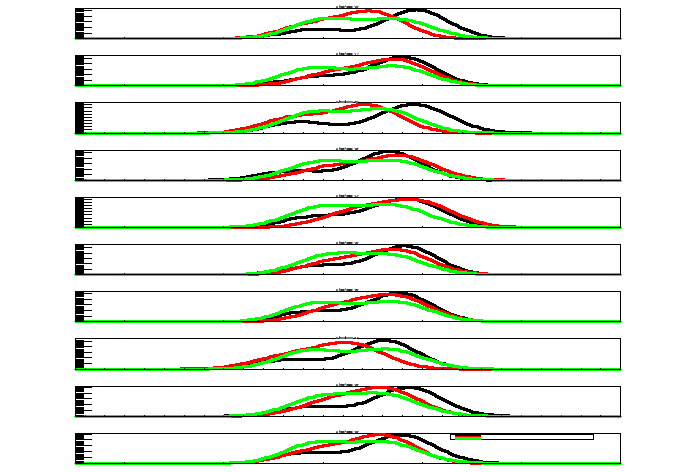
\includegraphics[width=14pc]{decomposed_model.pdf}
%\caption{\label{fig:unidist1} The component distributions.} %,$p_0(x)$, $p_1(x)$ and $p_2(x)$.}
%\end{minipage}\hspace{2pc}%
%\begin{minipage}{14pc}
%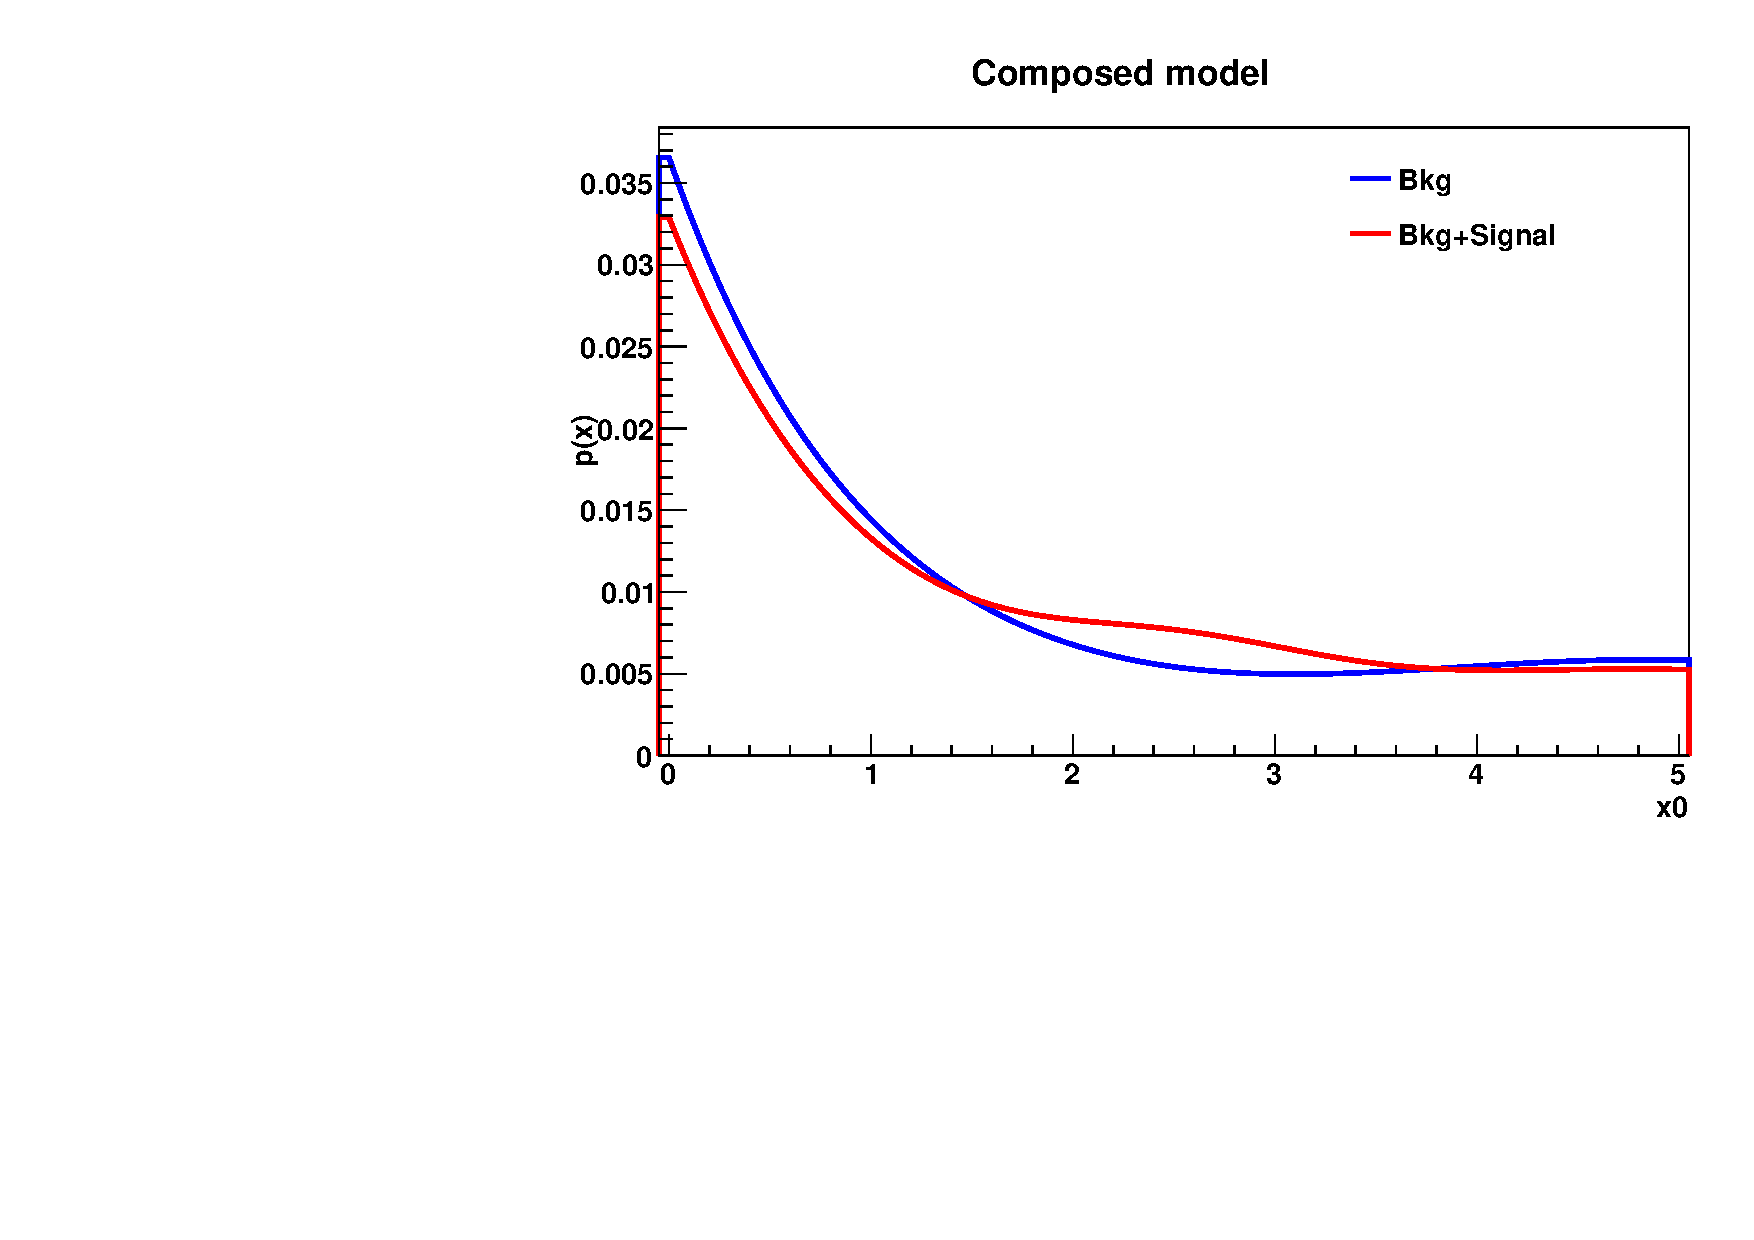
\includegraphics[width=14pc]{full_model.pdf}
%\caption{\label{fig:unidist2}The mixture models.}
%\end{minipage}
%\end{figure}
 
%In section 4.1 we present a simple case in which each one of the components is a standard univariate distribution. In section 4.2 we consider a harder mixture model consisting of three distributions, each one composed by the sum of three multivariate gaussian distributions.  In both cases all studies were conducted using a simple multilayer perceptron model. This classifier shows a good tradeoff between quality of the ratios and simplicity of the model. Others classifiers tested were boosted decision trees, logistic regression and support vector machines, all giving relatively good results. The probability models were implemented with \texttt{RooFit} probabilistic programming language and the classifiers were implemented using \texttt{Theano}(a framework to build neural network models) and \texttt{scikit-learn}(a general framework for machine learning in python)~\cite{Verkerke:2003ir,bergstra:2010-scipy,scikit-learn}.
%\subsection{Univariate Case}
%\subsubsection{Decomposing Likelihood Ratios}
%We consider a mixture model consisting of three distributions, $p_0(x)$ and $p_1$(x) are univariate gaussian distributions while $p_2(x)$ is a decaying exponential. The mixture models are composed by the weighted sum of those distributions where $p_0(x)$ correspond to the signal component.  The single distributions and the mixture models with coefficients $W(\theta_0) = \{0., 0.3, 0.7\}$ for the only background hypothesis and $W(\theta_1) = \{0.1, 0.27, 0.63\}$ for the background plus signal hypothesis are shown in Figure~\ref{fig:unidist}.

\begin{figure}[h]
%\hspace{3pc}
\begin{minipage}{12pc}
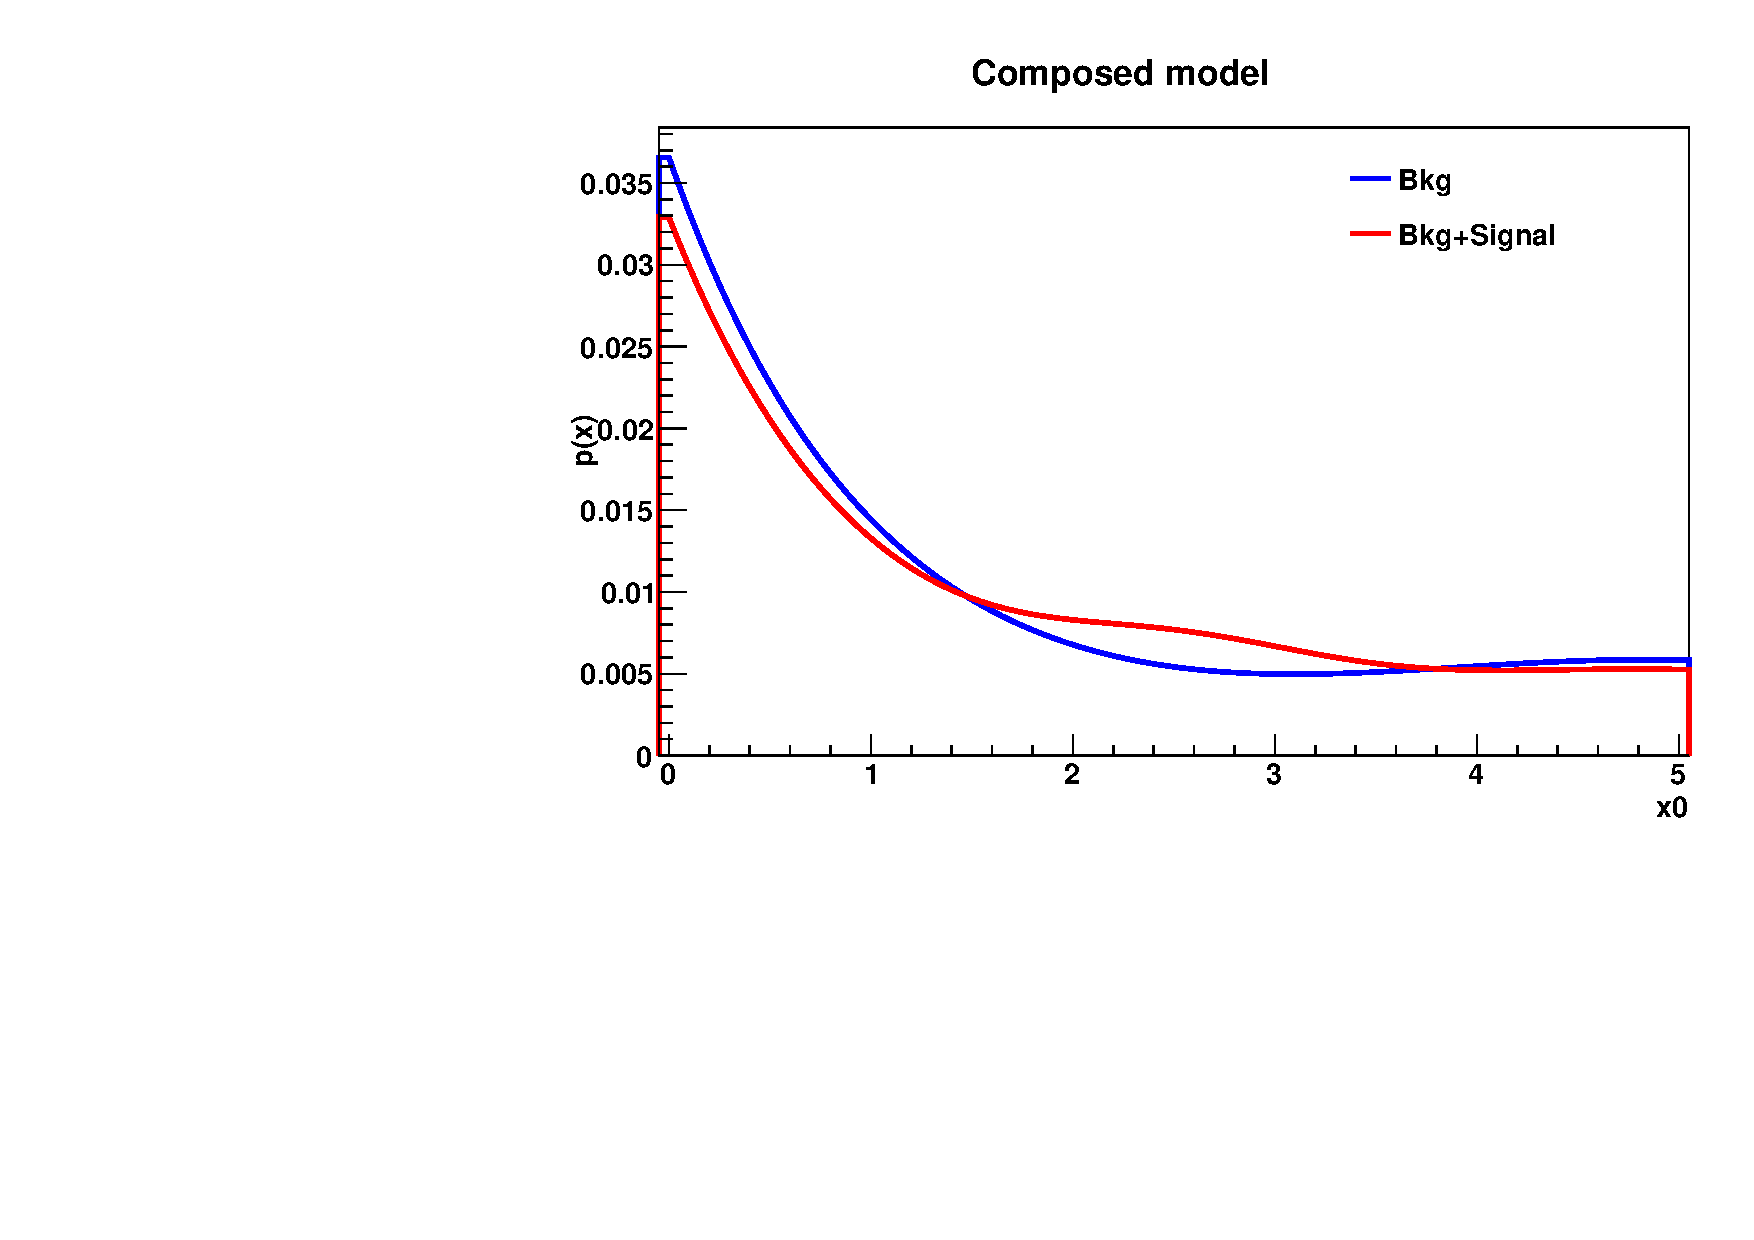
\includegraphics[width=12pc]{full_model.pdf}
\caption{\label{fig:unidist2}The mixture models.}
\end{minipage}\hspace{1pc}
\begin{minipage}{12pc}
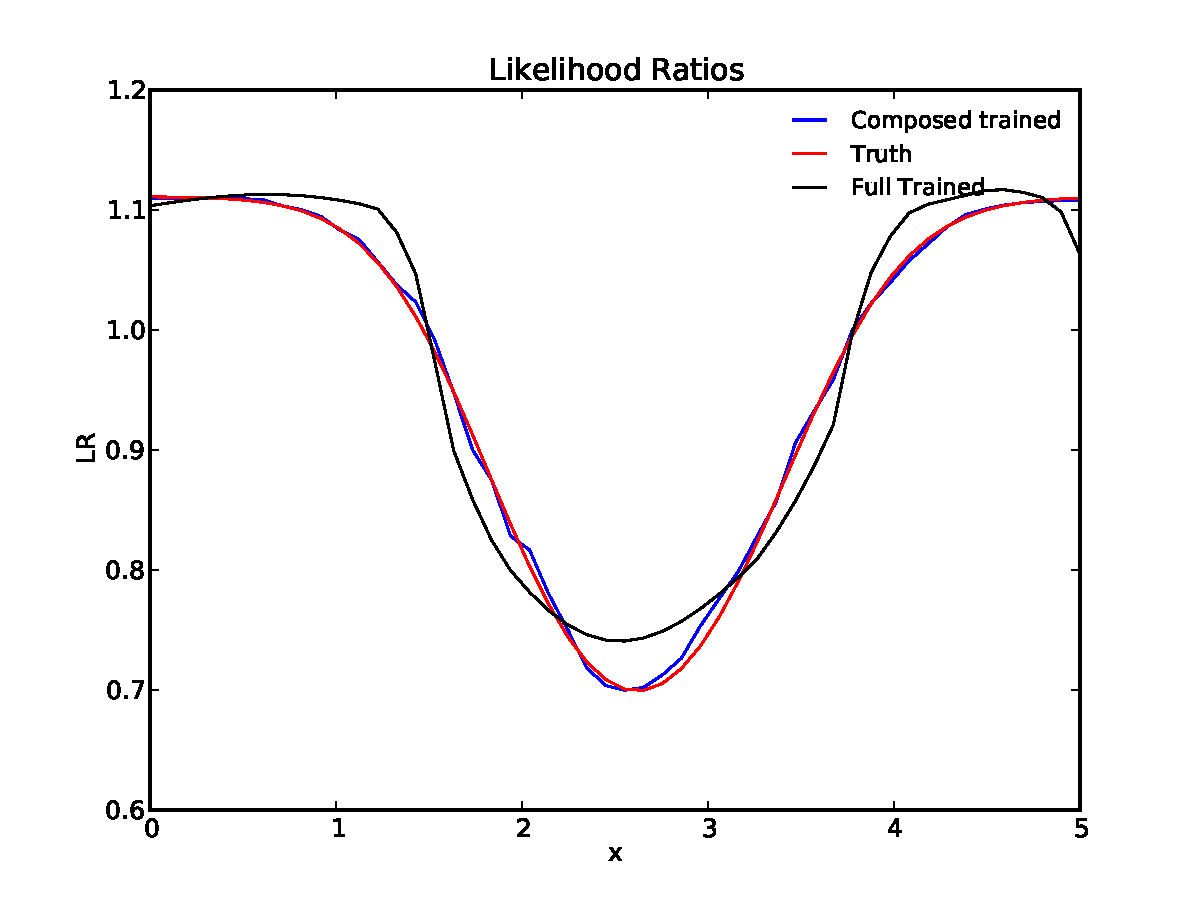
\includegraphics[width=12pc]{all_train_mlp_ratio_01.pdf}
\caption{\label{fig:ratios1} Density ratio comparison for a signal weight of $0.1$.} %,$p_0(x)$, $p_1(x)$ and $p_2(x)$.}
\end{minipage}\hspace{1pc}%
\begin{minipage}{12pc}
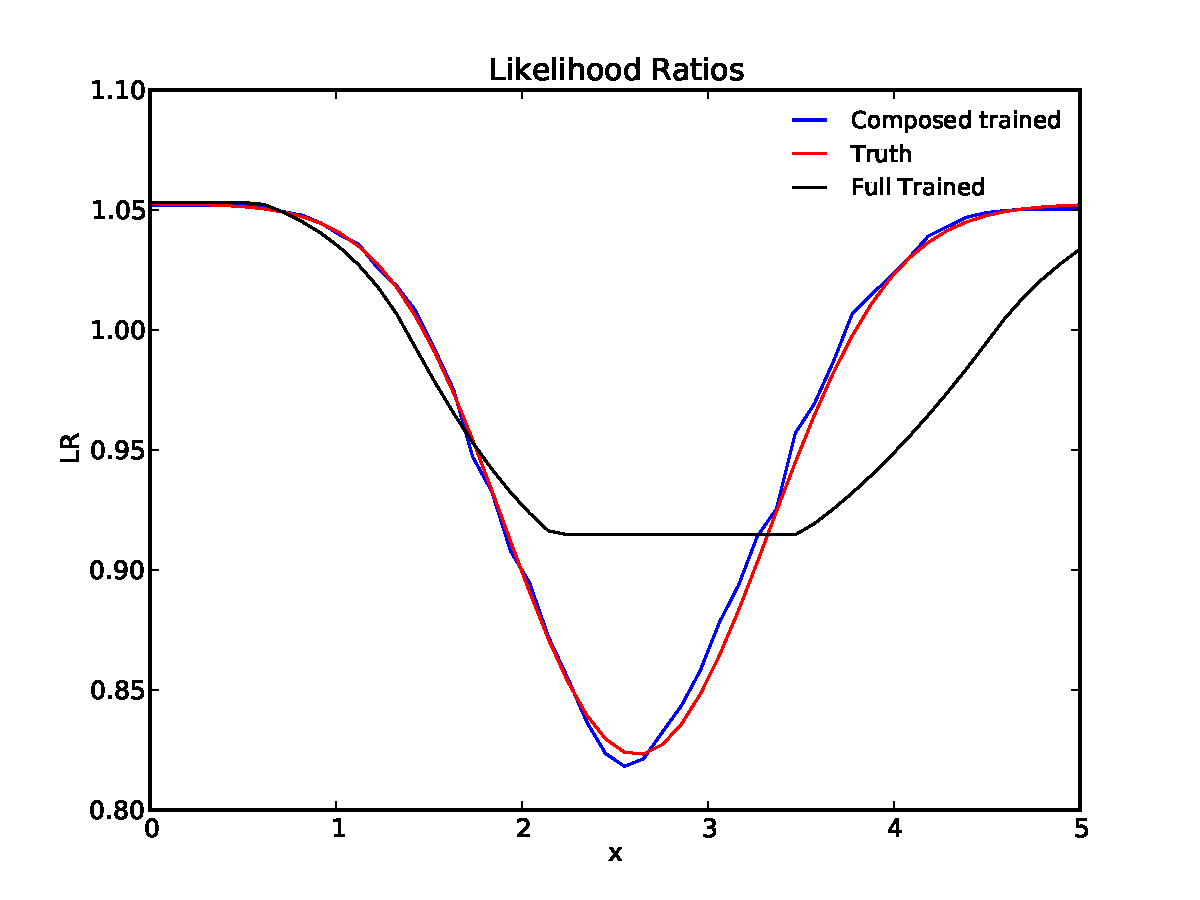
\includegraphics[width=12pc]{all_train_mlp_ratio_05.pdf}
\caption{\label{fig:ratios2} Density ratio comparison for a signal weight of $0.05$.}
\end{minipage}
\end{figure}

Three neural networks were trained on 200000 examples sampled from the pairs of single distributions and one on 200000 examples sampled from the full model (is important to use the same amount of training data in order to allow a fair comparison). The distribution of the score is estimated using histograms (the number of bins were carefully chosen in order to allow a good approximation while minimizing poisson fluctuations). The composed ratio using 
eq.~(\ref{eq:decomp}), the ratio estimated using a classifier trained on data from the full model and the true density ratio are shown in Figure~\ref{fig:ratios1} and Figure~\ref{fig:ratios2} for different values of the signal contribution ($0.1$ and $0.05$) while keeping the ratio between the background contributions fixed. 

It can be seen that the ratios obtained by the composition method are better (closer to the true ratios) than the obtained using a model trained on data from the full mixture model and this become clearer when the signal contribution is smaller.

\begin{figure}[h]
\hspace{3pc}
\begin{minipage}{14pc}
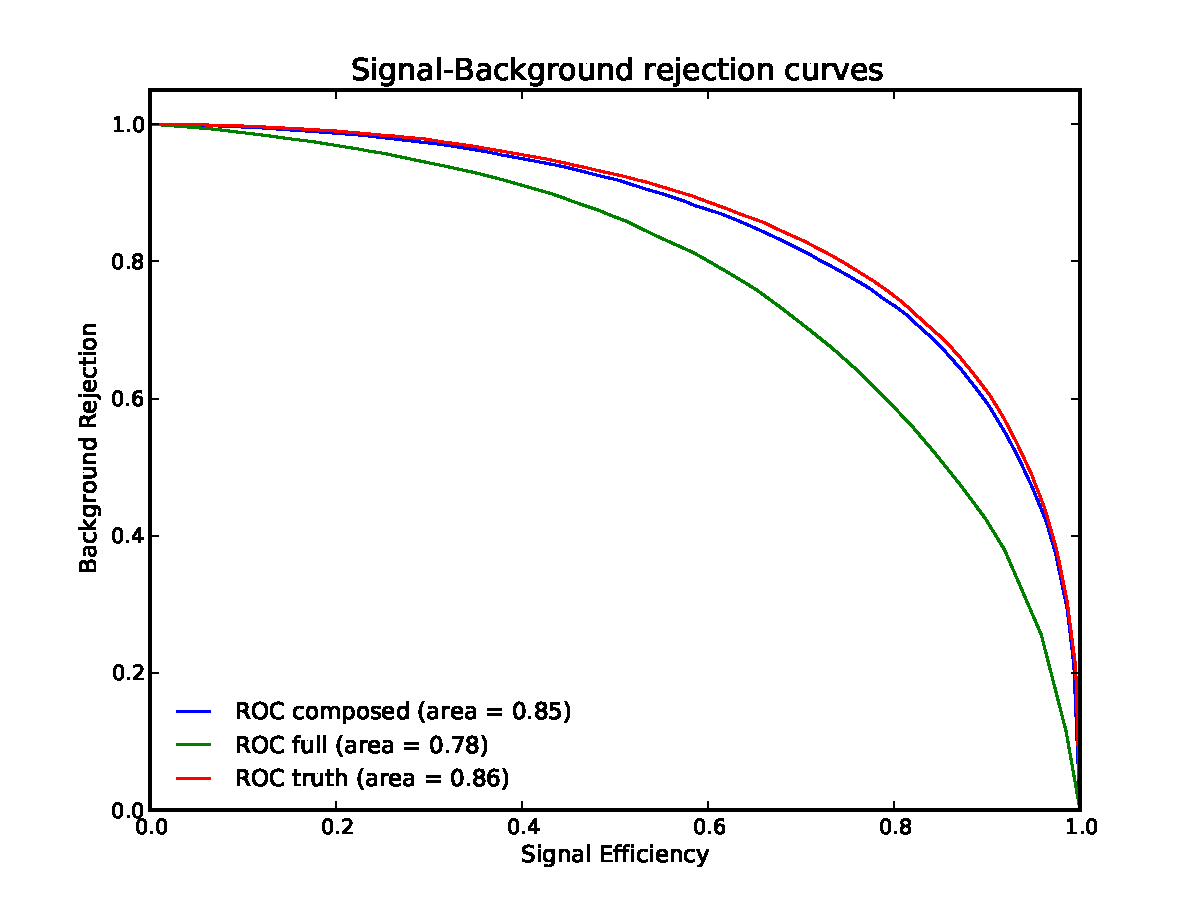
\includegraphics[width=14pc]{comp_all_mlp_sigbkg_01.pdf}
\caption{\label{fig:roc1} Background rejection versus signal efficiency curve comparison for a signal weight of $0.1$.} %,$p_0(x)$, $p_1(x)$ and $p_2(x)$.}
\end{minipage}\hspace{2pc}%
\begin{minipage}{14pc}
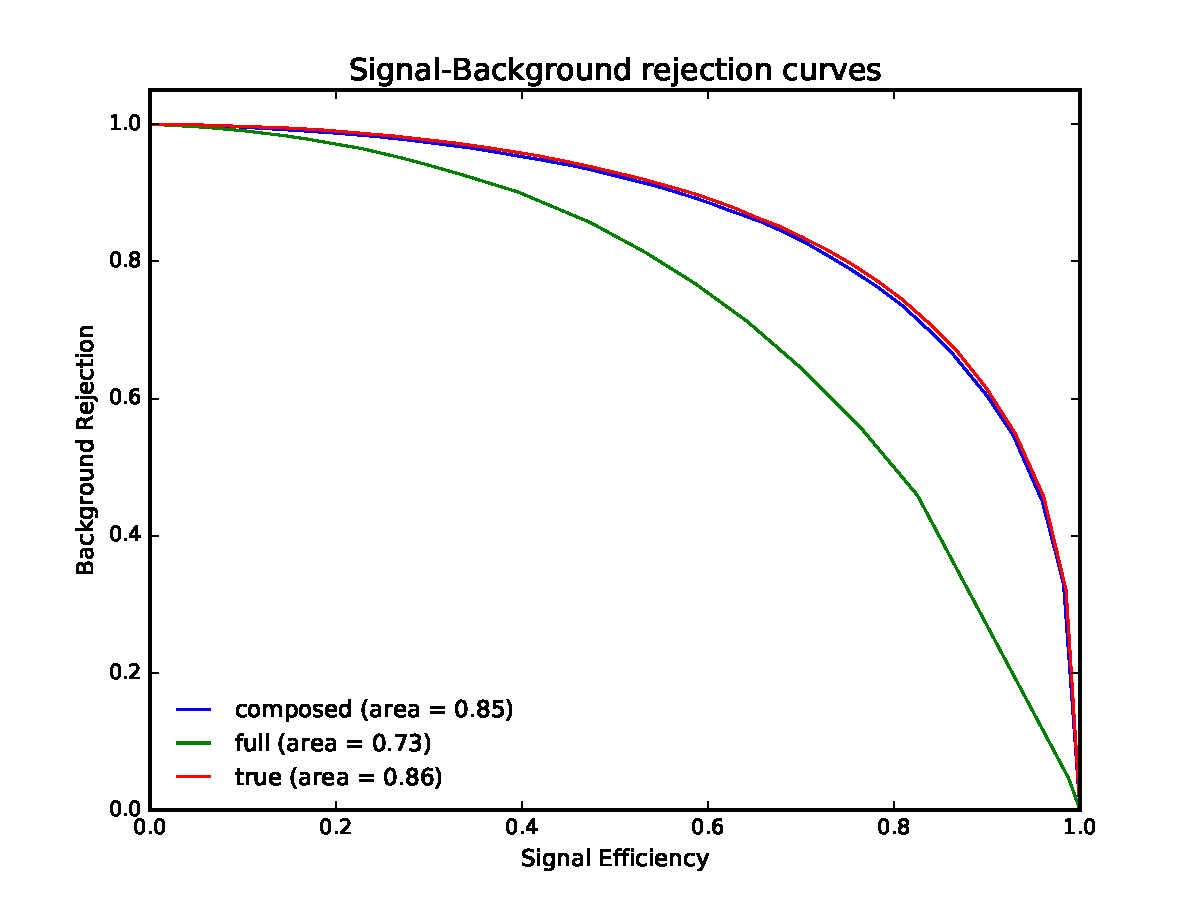
\includegraphics[width=14pc]{comp_all_mlp_sigbkg_005.pdf}
\caption{\label{fig:roc2} Background rejection versus signal efficiency curve comparison for a signal weight of $0.05$.}
\end{minipage}
\end{figure}

The same experiments are repeated but now considering a much harder mixture model consisting of three distributions, each one composed by the sum of three 10-dimensional multivariate gaussian distributions. In this case datasets of size 500000 were used to train all the models. This is more similar to what can be found in real physics experiments. To evaluate the estimated ratios the background rejection versus signal efficiency curves on data from $\theta_0$ and $\theta_1$ are used, employing the density ratio as discriminative variable. Again, the values for each one of the three cases (decomposed, full and true) are shown for a signal contribution of $0.1$ and $0.05$ in Figure~\ref{fig:roc1} and Figure~\ref{fig:roc2}.



The values of each one of the coefficients of the mixture model can be estimated by using the method of maximum likelihood as explained in Section~\ref{S:DLR}. In Figure~\ref{fig:2dfit} the contour plot for the likelihood ratio values given the signal and one background weight, obtained using the estimated density ratios and the true density ratios is shown. Histogram for the fitted values (estimated and true) of each one of the coefficients on 80 different pseudo-datasets of size 1000 are shown in Figure~\ref{fig:hist1} and Figure~\ref{fig:hist2}. It can be seen on the histograms that the estimations are unbiased.

\begin{figure}[h]
\begin{minipage}{11pc}
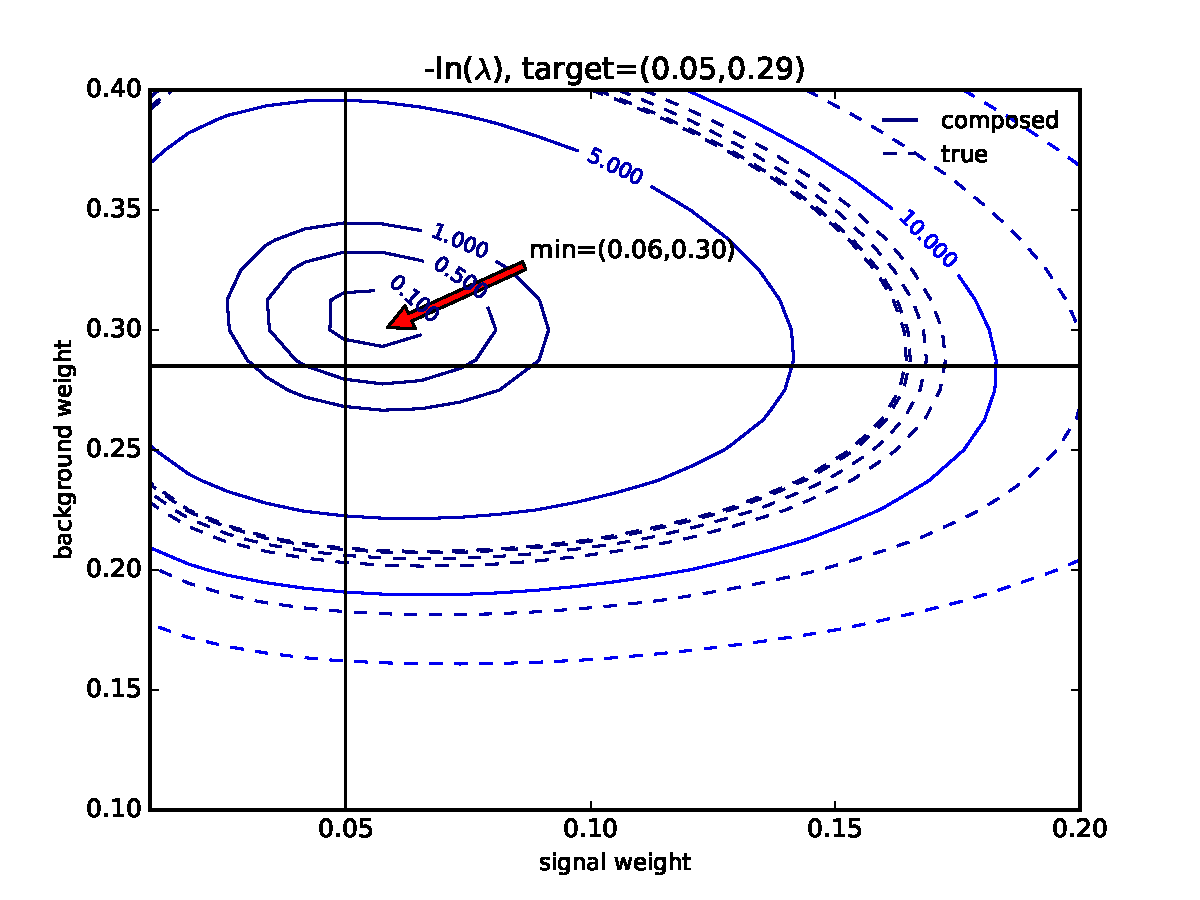
\includegraphics[width=12pc]{comp_train_mlp_multilikelihood.pdf}
\caption{\label{fig:2dfit} Likelihood ratio values given signal (c1[0]) and bkg. (c1[1]) weights.} %,$p_0(x)$, $p_1(x)$ and $p_2(x)$.}
\end{minipage}\hspace{2pc}%
\begin{minipage}{11pc}
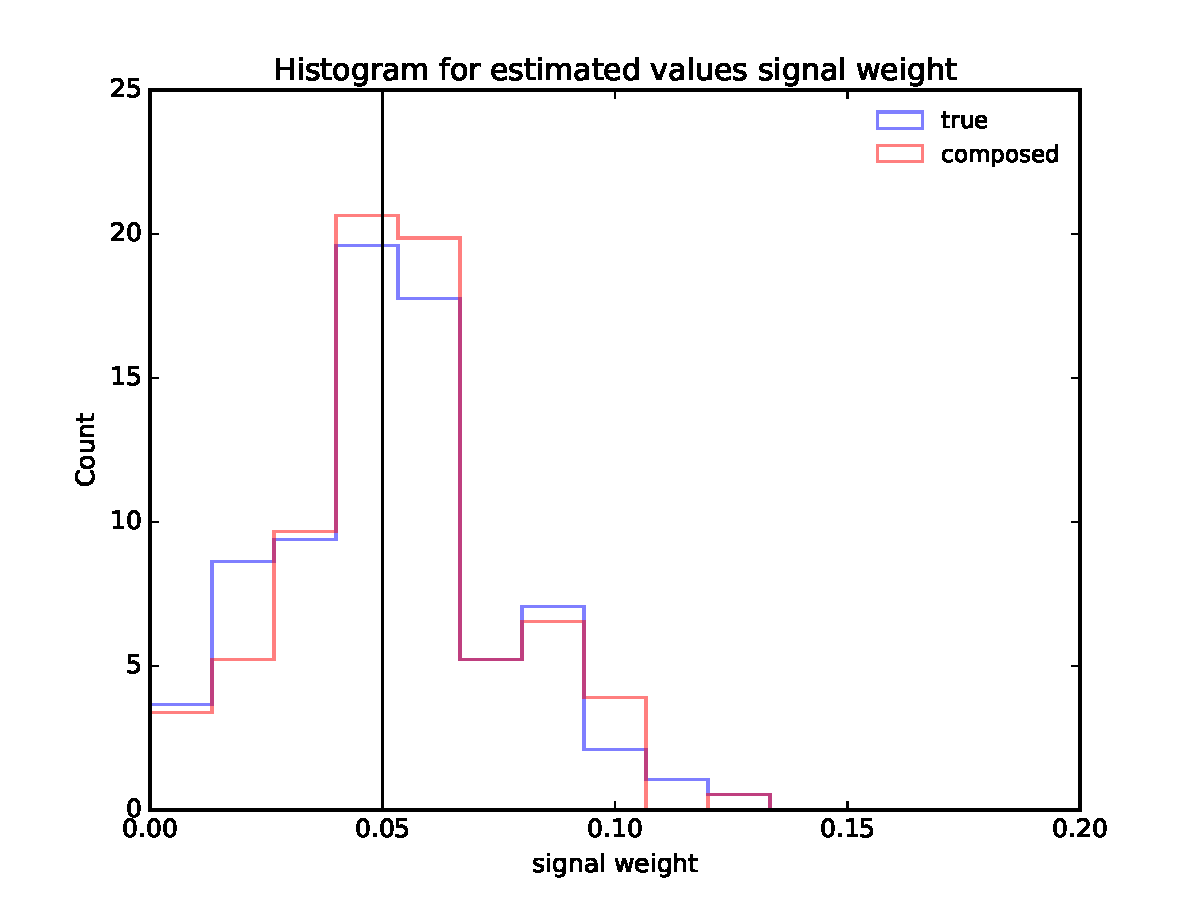
\includegraphics[width=12pc]{c1c2_train_mlp_c1_hist.pdf}
\caption{\label{fig:hist1} Histogram of fitted values for the signal weight (c1[0]).}
\end{minipage}\hspace{2pc}
\begin{minipage}{11pc}
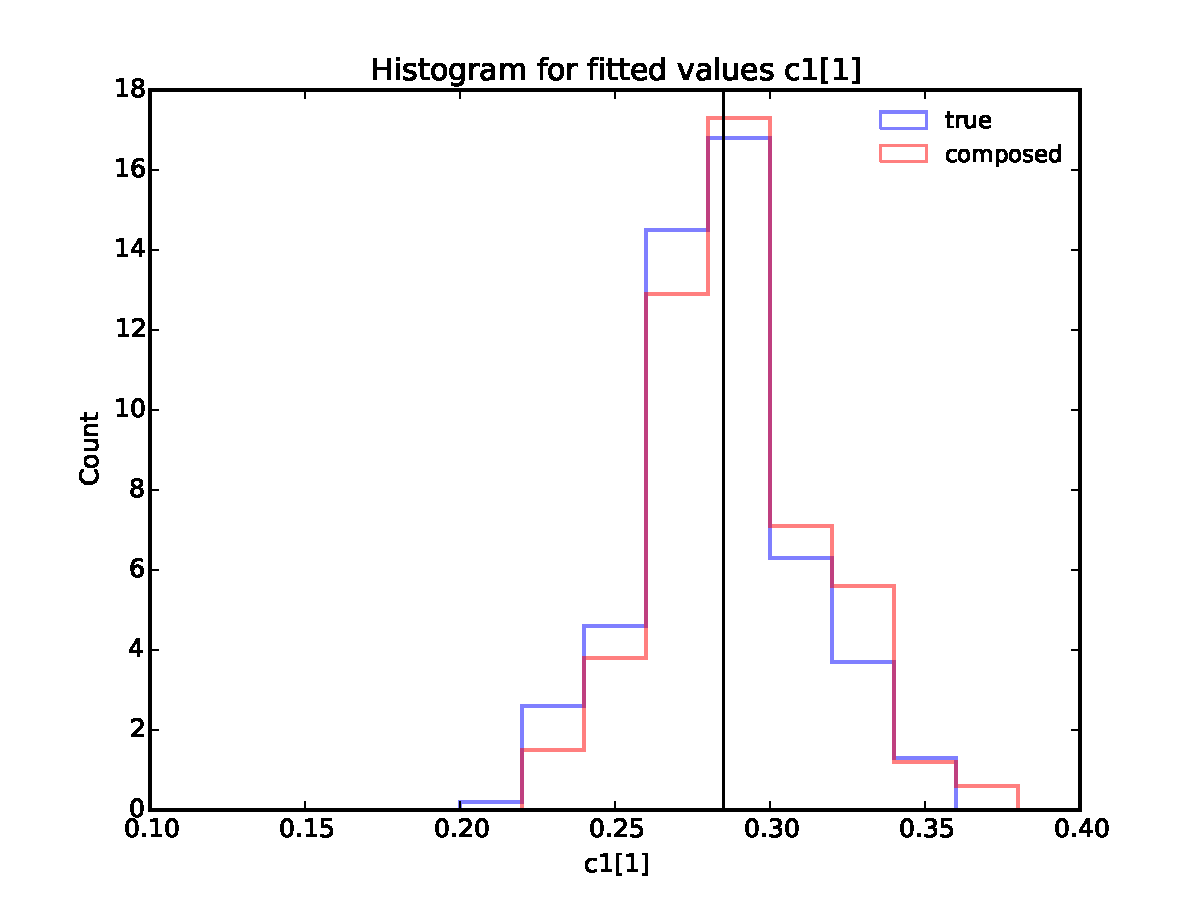
\includegraphics[width=12pc]{c1c2_train_mlp_c2_hist.pdf}
\caption{\label{fig:hist2}  Histogram of fitted values for the bkg. weight (c1[1]).}
\end{minipage}
\end{figure}

%Three neural networks composed by one hidden layer with 4 units are trained in 50000 samples (25000 samples generated from each component distribution) for the pairs $(p_0,p_1)$, $(p_0, p_2)$ and $(p_1,p_2)$. The distributions $p_i(s_{i,j}(x;\theta_0, \theta_1) |\theta)$ are estimated using histograms (kernel density estimation did not improved the results in this case). In this step some considerations must be carefully studied. When constructing the histograms, the number of bins used will affect the final approximation. Few bins will create bad estimations of the score distribution, on the other hand, many bins can produce better a better approximation but also (depending on the number of data used to construct the histograms) can create a noisy approximation due to poisson fluctuations. For a score with values ranging from $0$ to $1$, using 100000 samples in the histogram construction, it has been found that 40 bins gives a good tradeoff between quality of the estimation while minimizing the poisson noise. The ROC curves for each one of the pairwise trained classifiers using the approximated likelihood ratio $p_j(s_{i,j}(x;\theta_0,\theta_1)|\theta_1)/p_i(s_{i,j}(x;\theta_0, \theta_1)|\theta_0)$ as discriminative variable and the ROC curves obtained using the true likelihood ratio $p_j(x) / p_i(x)$ as discriminative variable together with the values of both ratios for values of $x \in [0,5]$ are shown in Figure \ref{fig:uniroc}. As expected the results looks very good since the pairs of distributions are relatively easy to discriminate. Finally, the complete likelihood ratios can be composed using Eq. \ref{eq:composition} in data generated from the full mixture models. 
%We also train a multilayer perceptron using the same architecture than the one used in the composed case and in data from the background only and background plus signal mixture models in order to obtain the likelihood ratios $p(s(x;\theta_0,\theta_1)|\theta_1)/p(s(x;\theta_0,\theta_1)|\theta_0)$ using the same procedure used for each one of the pairwise ratios. In Figure \ref{fig:fullratios} both the ratios for values of $x\in[0,5]$ and the signal efficiency versus background rejection curve on data generated from $p(x|\theta_0)$(only background mixture model) and $p_0(x|\theta_1)$(signal component) for the ratios obtained from the composed formula using pairwise trained classifiers, the ratios obtained using the classifier trained in the full models and applying directly Eq. \ref{eq:lrtest} and the ratios obtained from the true distributions are shown. It is clear that the ratios obtained by the composition method are better (closer to the true ratios) than the obtained using models trained in data from the full mixture model. In this case the value for the signal component is relatively large ($0.1$), in the next section we will show how the difference between the composed ratio and the ratios obtained from the full training become much bigger as the signal contribution is reduced.

%\begin{figure}[h]
%\includegraphics[width=14pc]{name.eps}\hspace{2pc}%
%\begin{minipage}[b]{14pc}\caption{\label{label}Figure caption for a narrow figure where the caption is put at the side of the figure.}
%\end{minipage}
%\end{figure}

%\begin{figure}[htbp]
%\begin{center}
%\includegraphics[height=2.2in]{uni_all_comparison_mlp_roc.pdf}
%\includegraphics[height=2.2in]{uni_all_dec_train_mlp_ratio.pdf}
%\caption{Left: The ROC curves obtained using the likelihood ratios of the score (trained) and true distributions as discriminative variable. Right: The ratio obtained from both method (trained and true) for values of x ranging from $0$ to $5$.  }
%\label{fig:uniroc}
%\end{center}
%\end{figure}

%\begin{figure}[htbp]
%\begin{center}
% \includegraphics[height=2.2in]{uni_all_train_mlp_ratio.pdf}
% \includegraphics[height=2.2in]{uni_comp_all_mlp_sigbkg.pdf}
%\caption{Left: The ratios obtained from each one of the methods (pairwise trained, full trained and full) for values of x ranging from $0$ to $5$. Right: The signal efficiency versus background rejection plots for each one of the method on data from the background model and the signal component. }
%\label{fig:fullratios}
%\end{center}
%\end{figure}

\section{Conclusions}
We have shown the power of using discriminative classifiers in order to approximate the likelihood ratio. In the case of mixture models we proved that the decomposed version of the ratio can greatly improve the quality of the results. Using the same method it was shown how to estimate the unknown parameters of the model. Initial experiments have been conducted on simulated data from different Higgs production mechanisms obtaining encouraging results. An open source \texttt{Python} package was implemented allowing to easily use the presented method (the package can be found at \url{https://github.com/diana-hep/carl}).
\section{Acknowledgments}
KC and GL are supported by the DIANA grant ACI-14503. JP was partially supported by the Scientific and Technological Center of Valparaiso (CCTVal) under Fondecyt grant BASAL FB0821. JP would like to thank Hector Allende and Carlos Valle for helpful discussions.


\section*{References}
\bibliography{learning}

\end{document}


